\subsection{Overview}
\subsection{Component View}
\begin{figure}[H]
    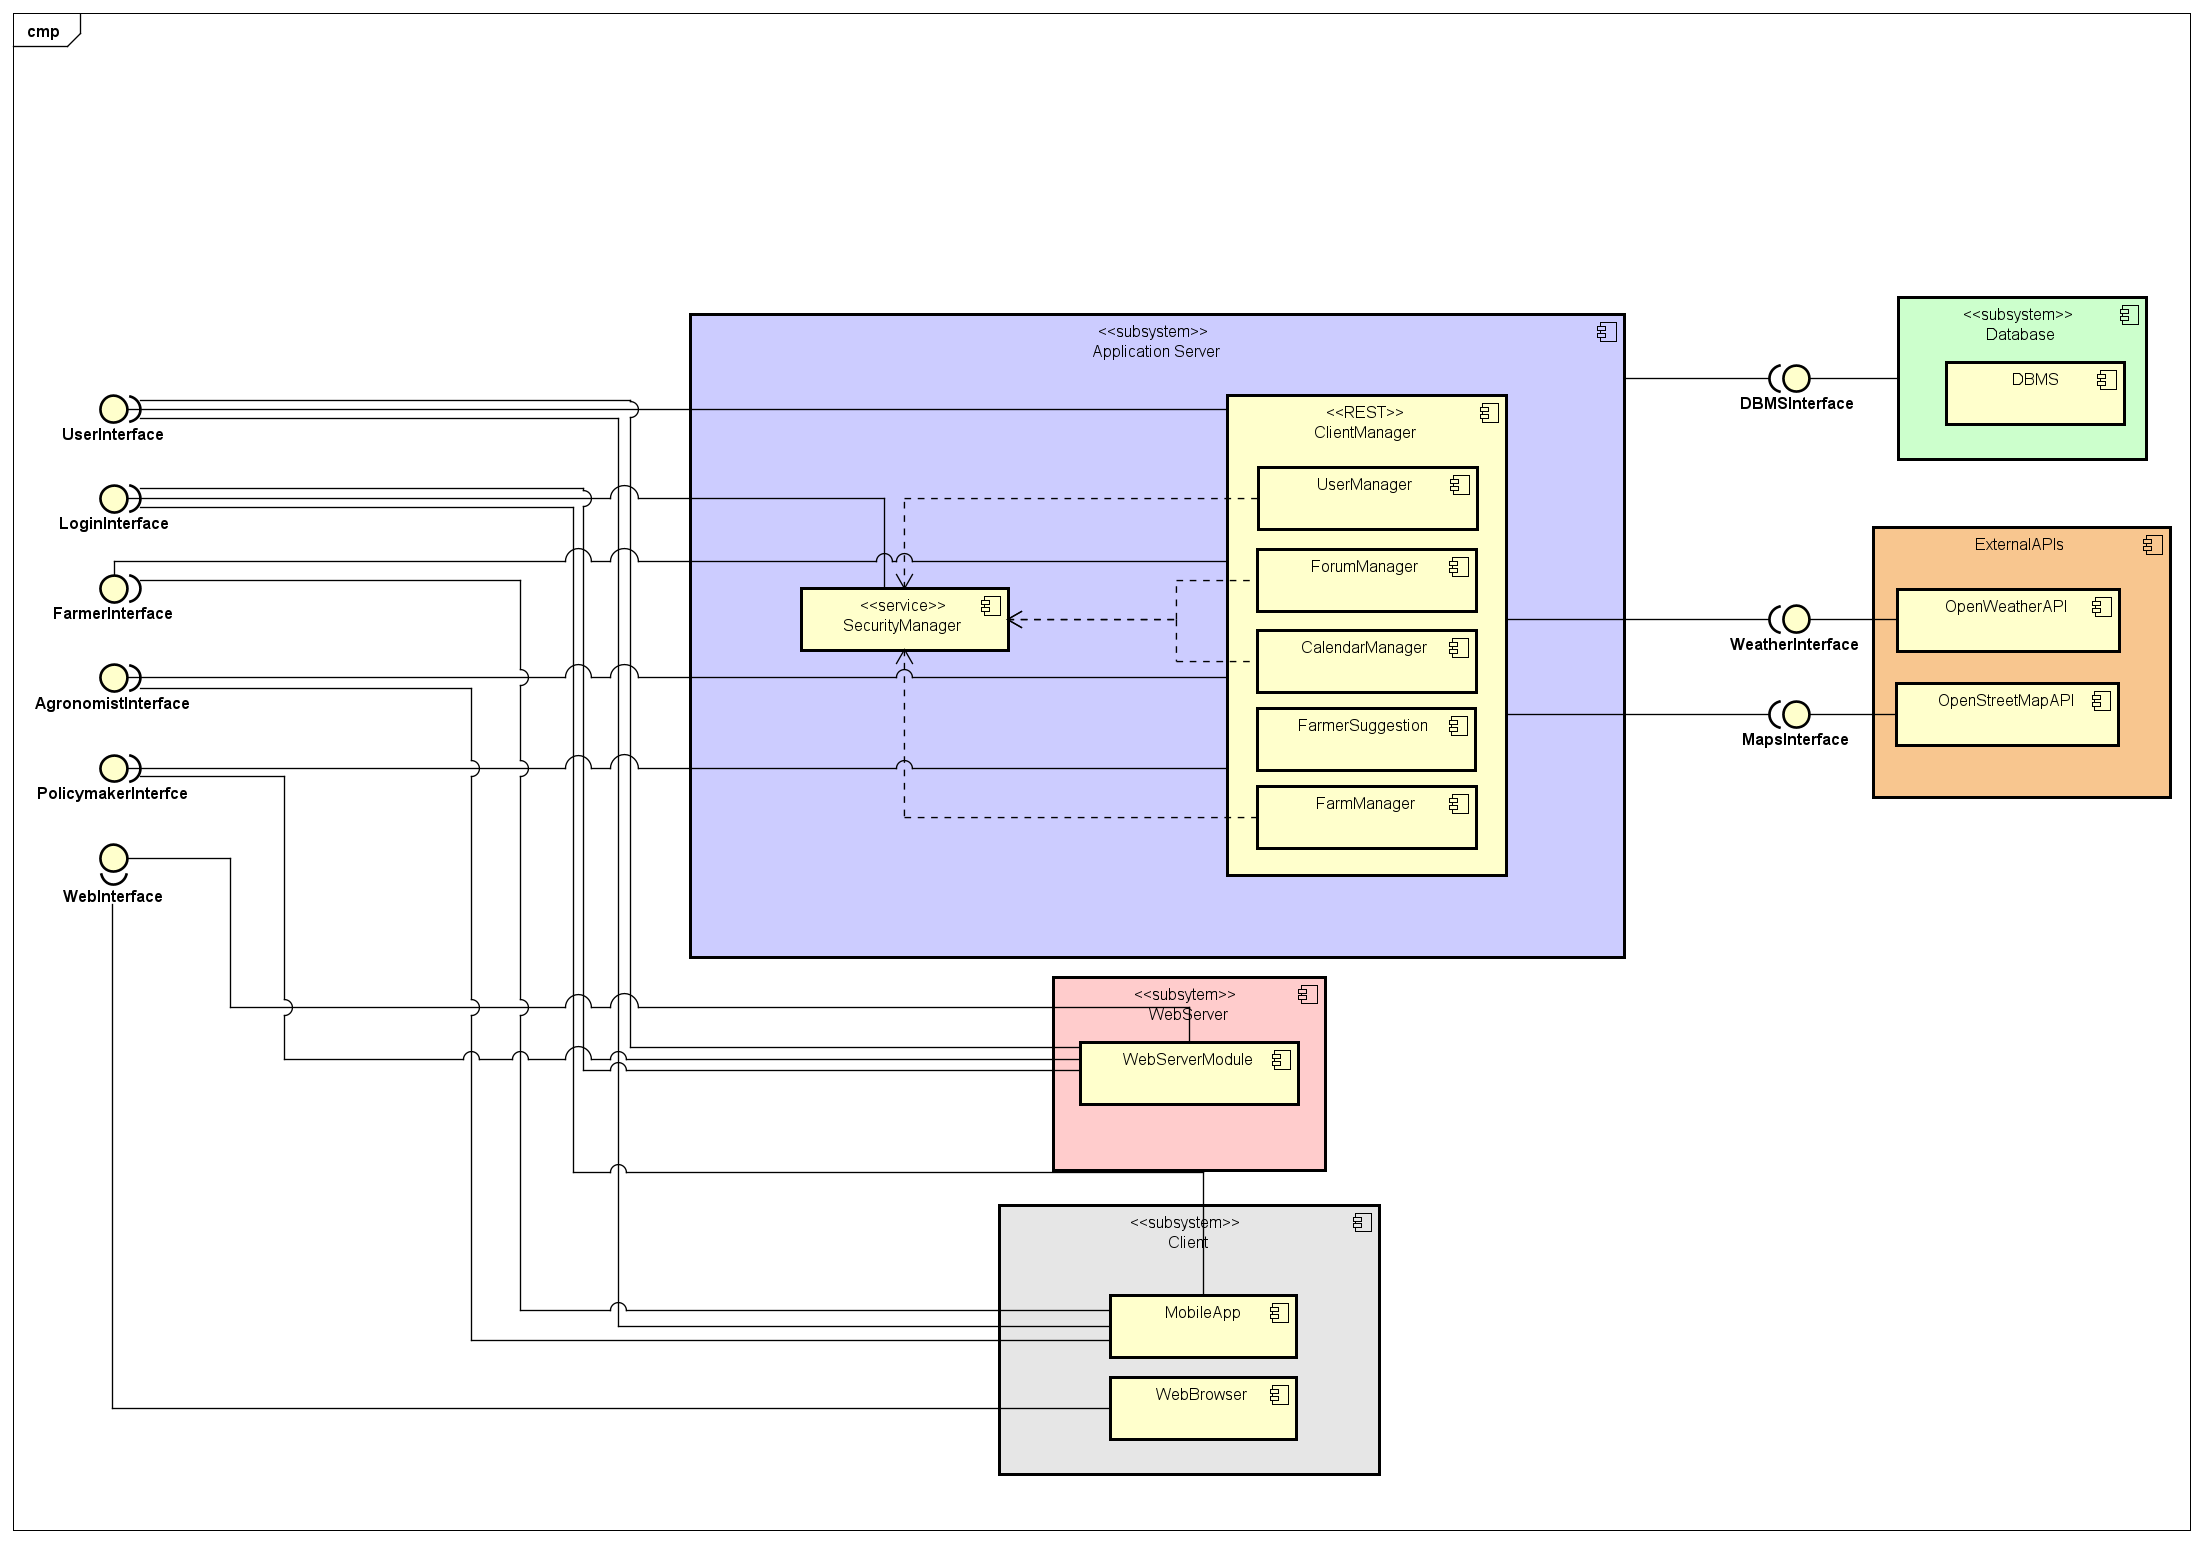
\includegraphics[width=\textwidth,height=\textheight,keepaspectratio]{Images/ComponentDiagram.png}
    \caption{Component Diagram}
    \label{fig:component_diagram}
\end{figure}

Figure \ref{fig:component_diagram}  represents in detail the layers described before. The web server has the funtion
route the browser requests to the application server and send back its responses.

\begin{itemize}
    \item \textbf{Client Manager}\\
        This module handles all the requests made by the client. In the beginning,
        when the client is not logged in, the module offers (through
        the user manager) a loginInterface that allows the client to register and log in. After the login the module
        provide an interface based on the role of the user: FarmInterface for the farmer, AgronomistInterface for the agronomist,
        PolicymakerInterface for the policymaker.

    \item \textbf{User Manager}\\
        This module provides all the functionalities needed to manage the user. It includes signup and login as well as role checking 
        operation and information retrieving.
           
    \item \textbf{Forum Manager}\\
        This module provides all the functionalities through the ForumInterface for managing and using the forum. 
        It includes operations for creating and replying to a discussion on the forum.

    \item \textbf{Calendar Manager}\\
        This Module provides all the functionalities needed for the Agronomist to manage his calendar. In particular, it provides
        through, the AgronomistInterface, the possibility to add or remove an appointment, to confirm the daily plan and to check
        that each farm has at least two visits per year.

    \item \textbf{Farmer Suggestion}\\
        This module handles the creation and delivery of personalized suggestions to the Farmer. 

    \item \textbf{Farm Manager}\\
        This module provides to the Farmer all the functionalities for giving information about their farm. 
        It provides the possibility to add information about the harvest and to request help from the Agronomist.

    \item \textbf{Security Manager}\\
        This module handles all the security issues.
\end{itemize}

\subsection{Logical Description of Data}
\begin{figure}[H]
    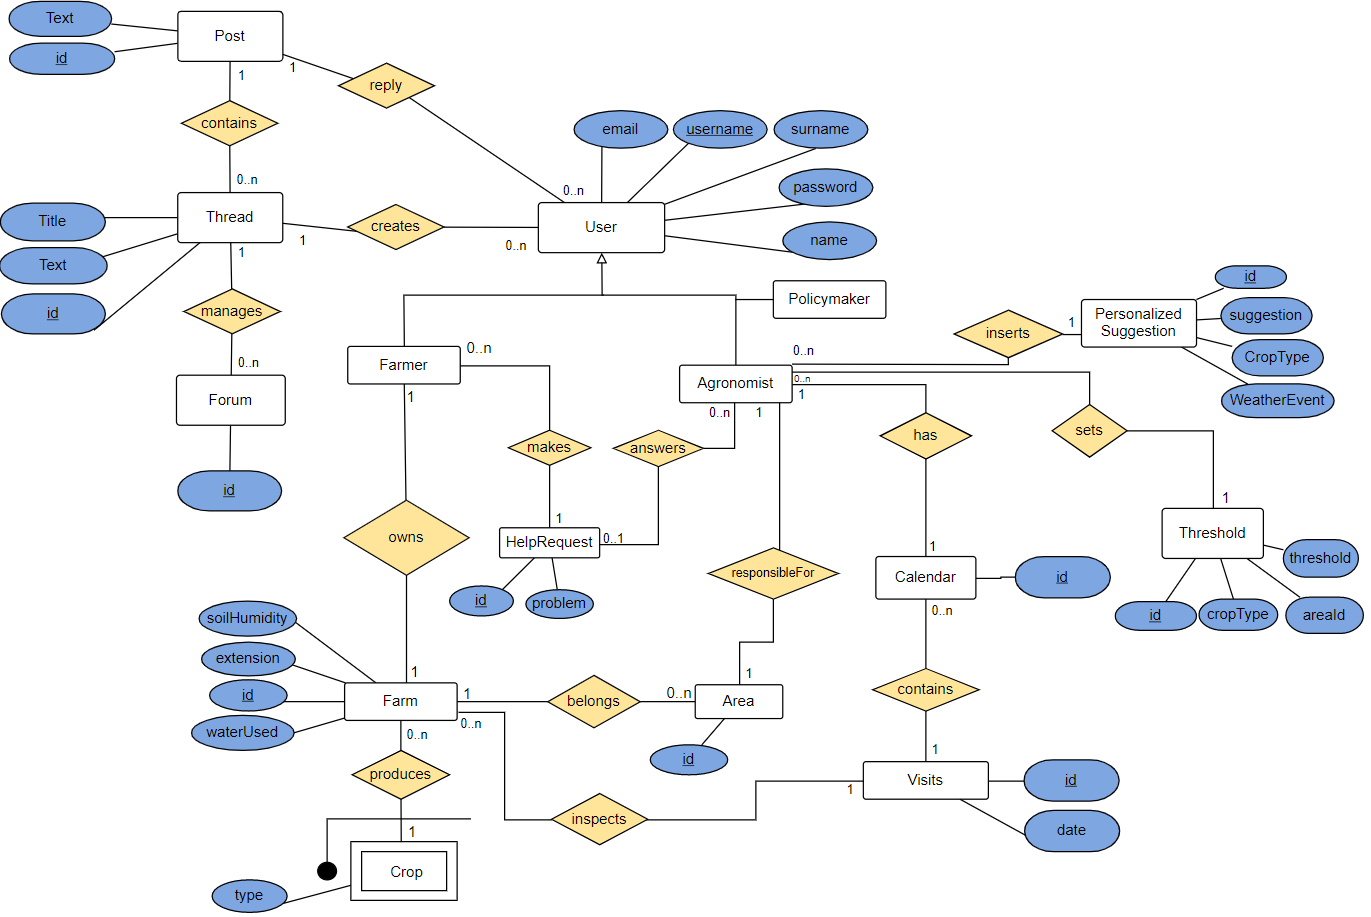
\includegraphics[width=\textwidth,height=\textheight,keepaspectratio]{Images/erDiagram.png}
    \caption{ER Diagram}
    \label{fig:er_diagram}
\end{figure}
